% !TeX root = RJwrapper.tex

\title{\pkg{JMcmprsk}: An R Package for Joint Modelling of
Longitudinal and Survival Data with Competing Risks}
\author{by Hong Wang, Ning Li, Shanpeng Li, and Gang Li}

\maketitle

\abstract{
In this paper, we describe an R package named \textbf{JMcmprsk}, for joint modelling of longitudinal and survival data with competing risks. The package in its current version implements two joint models of longitudinal and survival data proposed to handle competing risks survival data together with continuous and ordinal longitudinal outcomes respectively \citep{elashoff2008joint,li2010joint}. The corresponding R implementations are further illustrated with real examples. The package also provides simulation functions to simulate datasets for joint modelling with continuous or ordinal outcomes under the competing risks scenario, which provide useful tools to validate and evaluate new joint modelling methods.}

%\end{document}

\section{Introduction}
Joint modeling of  longitudinal and survival data has drawn a lot of attention over the past two decades. Much of the research has been focused on data with a single event time and a single type of failure, usually under the assumption of independent censoring of event times \citep{tsiatis2004joint}. However, in some situations interest lies with competing risks data, where there is more than one possible cause of an event or where the censoring is informative \citep{williamson2008joint}. Typically, a standard linear mixed model or its extensions are used for the longitudinal submodel. Cause-specific hazards model with either unspecified  or spline baseline hazards are studied for the competing risk submodels.  Various types of random effects are assumed to account for the association between these submodels.

Despite various theoretical and methodological developments \citep{hickey2018joint,papageorgiou2019overview}, there are still limited software packages to deal with specific problems in the analysis of follow-up data in clinical studies. To our knowledge, currently, there are three related  CRAN R packages, namely \textbf{JM} \citep{rizopoulos2012joint}, \textbf{joineR} \citep{williamson2008joint}, and \textbf{lcmm} \citep{proust2017estimation}, which support the modeling of longitudinal and survival data with competing risks.

The \textbf{JM} package provides support for competing risks via the "CompRisk" option in the \texttt{jointModel()} function.  In \textbf{JM}, a linear mixed-effects submodel is modeled for the longitudinal part and a relative risk submodel is assumed for each  competing event. In the current version (1.4-8), only the piecewise proportional hazards model, where the log baseline hazard is approximated using B-splines, is supported for the survival component.  The \textbf{joineR} package fits the joint model \citep{williamson2008joint} for joint models of longitudinal data and competing risks using the \texttt{joint()} function. In their model, the time-to-event data is modeled using a cause-specific Cox proportional hazards regression model with time-varying covariates. The longitudinal outcome is modeled using a linear mixed effects model. The association is captured by a zero-mean shared latent Gaussian process. Parameters in the model are estimated using an Expectation Maximization(EM) algorithm.  The \textbf{lcmm} package  implements the support for competing risks joint modeling in the \texttt{Jointlcmm()} function. Radically different from the above two R packages, the \textbf{lcmm} package  uses a less well-known framework called the joint latent class model \citep{proust2014joint}, which assumes that dependency between the longitudinal markers and the survival risk can be captured by a latent class structure entirely. However, the \textbf{lcmm} package is mainly designed for prediction purpose and may not be suited to evaluate specific assumptions regarding the characteristics of the marker trajectory that are the most influential on the event risk \citep{proust2014joint}.

In all these packages, a time-independent shared random effects vector is usually assumed in modeling the longitudinal and survival data. However, they are not capable of fitting more flexible models with separate random effects in these submodels \citep{elashoff2008joint,li2010joint}.  In many biomedical applications, sometimes, it is necessary to have a model which takes into account longitudinal ordinal outcomes for the longitudinal part. Yet, due to the complex nature of joint modeling, most of the available software does not support longitudinal ordinal variables \citep{armero2016bayesian, Ferrer2017phd}.   We thus decided to fill this gap and implemented a joint model which supports ordinal disease markers based on our previous work \citep{li2010joint}.

Both \textbf{JM} and \textbf{joineR} packages depend heavily on the R \textbf{nlme} and \textbf{survival} packages. In \textbf{JM}, the linear mixed-effects submodel and the survival submodel are first fitted using\texttt{ lme()} and \texttt{coxph()} R function in these packages before a joint modeling process. In \textbf{joineR}, \texttt{lme()} and \texttt{coxph()} functions are applied to obtain initial values for parameters in the joint model, which are further estimated by an EM algorithm. The major advantage of using available packages such as \textbf{survival} and \textbf{nlme} lies that joint modeling R packages can be built quickly with adequate efficiency as most of these base R packages have been optimized for speed.  However, if required functionality is not available in these packages, as is the case of \cite{elashoff2008joint} and \cite{li2010joint}, implementing new joint modeling methods is a non-trivial task.

Compared with \textbf{JM} and \textbf{joineR} packages, the \textbf{JMcmprsk} package introduced here can be regarded as a "stand-alone" R package, which does not required initial estimates for the linear mixed effects model or survival submodel to compute parameters of the joint model in question. In particular, the \textbf{JMcmprsk} package is built within the \textbf{Rcpp} \citep{eddelbuettel2011rcpp} and \textbf{GSL}(The GNU Scientific Library)\citep{galassi2002gnu} framework, which make R functions have access to a wide range of fast numerical routines such as Monte Carlo integration, numerical integration and differentiation.

 \section{ Joint Models with Competing Risks }
 A joint model for competing risk data consists of two linked components: the longitudinal submodel, which takes care of repeatedly measured information and the survival submodel, which deals with multiple failure times. The combination of different longitudinal and survival components leads to a variety of joint models \citep{hickey2018comparison}.

 In the current version of \textbf{JMcmprsk}, we have implemented two joint models for competing risk data, namely joint modeling with continuous longitudinal outcomes \citep{elashoff2008joint}, and joint modeling with ordinal longitudinal outcomes \citep{li2010joint}. Both models have adopted a cause-specific Cox submodel with a frailty term for multiple survival endpoints. The difference between these two models lies in the longitudinal part.  The former model applies a linear mixed submodel for the continuous longitudinal outcome, while the latter model includes a partial proportional odds submodel for the ordinal longitudinal outcome.

 Different from previous approaches \citep{rizopoulos2012joint,williamson2008joint}, we assume a flexible separate random effects structure for the longitudinal submodel and the survival submodel. Furthermore, the association between both submodels is modeled by the assumption that the random effects in two submodels jointly have a multivariate normal distribution.

\subsection{Model 1: Joint modeling with continuous longitudinal outcomes}

Let $Y_i(t)$ be the longitudinal outcome measured at time $t$ for subject $i$, $i=1,2,\cdots,n$ and $n$ is the total number of subjects in study. Let $C_i=(T_i,D_i)$ denote the competing risks data on subject $i$, where $T_i$ is the failure time or censoring time, and $D_i$ takes value in $\{0,1,\cdots,g\}$, with $D_i=0$ indicating a censored event and $D_i=k$ showing that subject $i$ fails from the $k$th type of failure, where $k=1,\cdots,g$.

The joint model is specified in terms of the following two linked submodels:
\begin{eqnarray*}
Y_i(t)&=&X_i^{(1)}(t)^\top \beta+\tilde X_i^{(1)}(t)^\top b_i+\epsilon_i(t),\\
\lambda_k(t)&=&\lambda_{0k}(t)\exp(X_i^{(2)}(t)^\top \gamma_k+\nu_k u_i),~~\mbox{for}~~k=1,\cdots,g,
\end{eqnarray*}
where $X_i^{(1)}(t)$, $X_i^{(2)}(t)$ denote the covariates for the fixed-effects $\beta$ and $\gamma_k$, $\tilde X_i^{(1)}(t)$ denotes the covariates for the random-effects $b_i$ and $\epsilon_i(t)\sim N(0,\sigma^2)$ for all $t\geq 0$. The parameter $\nu_1$ is set to 1 to ensure identifiability. We assume that $b_i$ is independent of $\epsilon_i(t)$ and that $\epsilon_i(t_1)$ is independent of $\epsilon_i(t_2)$ for any $t_1\neq t_2$. We further assume the random effects $b_i$ and $u_i$ jointly have a multivariate normal distribution, denoted by $\theta_i\sim N(0,\Sigma)$, where $\Sigma=(\Sigma_{b},\Sigma_{bu}^\top;\Sigma_{bu},\sigma_u)$.

Denote $\Psi$ as the unknown parameters from the joint models. We propose to obtain the maximum likelihood estimate of $\Psi$ through an EM algorithm. The complete data likelihood is
\begin{eqnarray*}
&&L(\Psi;Y,C,\theta)\\
&&\propto \Pi_{i=1}^n\Big[\Pi_{j=1}^{n_i}\frac{1}{\sqrt{2\pi\sigma^2}}\exp(-\frac{1}{2\sigma^2}(Y_{ij}-X_i^{(1)}(t_{ij})^\top\beta-\tilde X_i^{(1)}(t_{ij})^\top b_i)^2)\Big]\\
&&\times \Pi_{k=1}^g\lambda_k(T_i)^{I(D_i=k)}\exp\Big\{-\int_0^{T_i}\sum_{k=1}^g\lambda_k(t)dt\Big\}\\
&&\times \frac{1}{\sqrt{(2\pi)^d|\Sigma|}}\exp(-\frac{1}{2}\theta_i^\top\Sigma^{-1}\theta_i).
\end{eqnarray*}

In the E-step, we need to calculate the expected value of all the functions of $\theta$. Since the integral over the random effects does not have a closed-form solution, an iterative numerical method has to be employed.

In \textbf{JMcmprsk}, the integral over time is approximated using a Gauss-Kronrod quadrature and the computation of the integral over the individual random effects is achieved using a Gauss-Hermite quadrature. The quadrature approximates the integral using a weighted sum of function values at specified points within the domain of integration; the Gaussian quadrature is based on the use of polynomial functions. A standard option here is the Gaussian quadratic rules. In the M-step, $\Psi$ is updated by maximizing the functions obtained from the E-step.

\subsection{Model 2: Joint modeling with ordinal longitudinal  outcomes}

Let $Y_{ij}$ denote the $j$th response measured on subject $i$, where $i=1,\cdots,n$, $j=1,\cdots,n_i$, and $Y_{ij}$ takes values in $\{1,\cdots,K\}$. The competing risks failure times on subject $i$ is $(T_i,D_i)$, and the notations have the same meaning as in Model 1.

We propose the following partial proportional odds model for $Y_{ij}$
\begin{eqnarray*}
P(Y_{ij}\leq k|X_{ij},\tilde X_{ij},W_{ij},b_i)=\frac{1}{1+\exp(-\theta_{k}-X_{ij}\beta-\tilde X_{ij}\alpha_{k}-W_{ij}^\top b_i)},
\end{eqnarray*}
where $k=1,\cdots,K-1$, $X_{ij}$ and $\tilde X_{ij}$ are $p\times 1$ and $s\times 1$ vectors of covariates for the fixed-effect $\beta$ and $\alpha_{k}$, with $\alpha_{1}=0$, and $\tilde X_{ij}$ is a subset of $X_{ij}$ for which the proportional odds assumption may not be satisfied. The $q\times 1$ vector $b_i$ represents random effects of the associated covariates $W_{ij}$.

The distribution of the competing risks failure times $(T_i,D_i)$ are assumed to take the form of the following cause-specific hazards frailty model:
\begin{eqnarray*}
\lambda_d(t|Z_i(t),u_i)&=&\lambda_{0d}(t)\exp(Z_i(t)^\top \gamma_d+\nu_d u_i),~~\mbox{for}~~d=1,\cdots,g,
\end{eqnarray*}
where the $l\times 1$ vector $\gamma_d$ and $\nu_d$ are the cause-specific coefficients for the covariates $Z_i(t)$ and the random effects $u_i$, respectively.

The parameter $\nu_1$ is set to 1 to ensure identifiability. We assume the random effects $b_i$ and $u_i$ jointly have a multivariate normal distribution, denoted by $a_i\sim N(0,\Sigma)$.

Denote $\Psi$ as the unknown parameters from the joint models. We propose to obtain the maximum likelihood estimate of $\Psi$ through an EM algorithm. The complete data likelihood is
\begin{eqnarray*}
&&L(\Psi;Y,C,a)\\
&&\propto \Pi_{i=1}^n\Big[\Pi_{j=1}^{n_i}\Pi_{k=1}^{K}\{\pi_{ij}(k)-\pi_{ij}(k-1)\}^{I(Y_{ij}=k)}\Big]\\
&&\times \Pi_{d=1}^g\lambda_d(T_i)^{I(D_i=d)}\exp\Big\{-\int_0^{T_i}\sum_{k=1}^d\lambda_d(t)dt\Big\}\\
&&\times \frac{1}{\sqrt{(2\pi)^{q+1}|\Sigma|}}\exp(-\frac{1}{2}a_i^\top\Sigma^{-1}a_i).
\end{eqnarray*}
where $\pi_{ij}(k)$ stands for the probability that $Y_{ij}\leq k$ given the covariates and the random effects. The implementation of EM algorithm in this case is similar to the procedure of Model 1.


\section{Package structure and functionality}

The R package \textbf{JMcmprsk} implements the above two joint models on the basis of R package \textbf{Rcpp} \citep{eddelbuettel2011rcpp}  and \textbf{GSL} library\citep{galassi2002gnu} and is hosted at CRAN. After setting the GSL environment by following the instructions in the INSTALL file from the package, we can issue the following command in the R console to install the package:

> install.packages("JMcmprsk")

There are two  major functions included in the \textbf{JMcmprsk} package: the function that fits continuous outcomes  \texttt{jmc()}  and the function that fits ordinal outcomes \texttt{jmo()}.

\subsection{jmc() function}
As an illustrative example of \texttt{jmc()}, we consider Scleroderma Lung Study \citep{tashkin2006cyclophosphamide}, a double-blinded, randomized clinical trial to evaluate the effectiveness of oral cyclophosphamide (CYC) versus placebo in the treatment of lung disease due to scleroderma. This study consists of 158 patients and the primary outcome is forced vital capacity (FVC, as \% predicted) determined at 3-month intervals from the baseline. The event of interest is the time-to-treatment failure or death. We consider two covariates, baseline \%FVC ($FVC_0$) and baseline lung fibrosis ($FIB_0$) and two risks, informative and noninformative. The model setups are as follows:
\begin{eqnarray*}
\%FVC_{ij}&=&\beta_0+\beta_1t_{ij}+\beta_2FVC_{0i}+\beta_3FIB_{0i}+\beta_4CYC_i\\
&&+\beta_5FVC_{0i}\times CYC_i+\beta_6FIB_{0i}\times CYC_i+\beta_7 t_{ij}\times CYC_i+b_it_{ij}+\epsilon,
\end{eqnarray*}
and the cause-specific hazards frailty models are
\begin{eqnarray*}
\lambda_1(t)=\lambda_{01}(t)\exp(\gamma_{11}FVC_{0i}+\gamma_{12}FIB_{0i}+\gamma_{13}CYC_i+\gamma_{14}FVC_{0i}\times CYC_i+\gamma_{15}FIB_{0i}\times CYC_i+u_i)\\
\lambda_2(t)=\lambda_{02}(t)\exp(\gamma_{21}FVC_{0i}+\gamma_{22}FIB_{0i}+\gamma_{23}CYC_i+\gamma_{24}FVC_{0i}\times CYC_i+\gamma_{25}FIB_{0i}\times CYC_i+\nu_2u_i),
\end{eqnarray*}


We first load the package and the data.
\begin{example}
library(JMcmprsk)
set.seed(123)
data(lung)
yread <- lung[, c(1,2:11)]
cread <- unique(lung[, c(1, 12, 13, 6:10)])
\end{example}
The number of rows in "yread" is the total number of measurements for all subjects in the study. For "cread", the survival/censoring time is included in the first column, and the failure type coded as 0 (censored events), 1 (risk 1), or 2 (risk 2) is given in the second column. Two competing risks are assumed.

Then, "yread" and "cread" are used as the longitudinal and survival input data for the model specified by the function \texttt{jmc() }as shown below:

\begin{example}
jmcfit <- jmc(long_data = yread, surv_data = cread, out = "FVC",
           FE = c("time", "FVC0", "FIB0", "CYC", "FVC0.CYC",
                  "FIB0.CYC", "time.CYC"),
           RE = "linear", ID = "ID",cate = NULL, intcpt = 0,
           quad.points = 20, quiet = TRUE, do.trace = FALSE)
\end{example}
where \texttt{out} is the name of the outcome variable in the longitudinal sub-model, \texttt{FE} the list of covariates for the fixed effects in the longitudinal sub-model, \texttt{RE} the types/vector of random effects in the longitudinal sub-model, \texttt{ID} the column name of subject id, \texttt{cate} the list of categorical variables for the fixed effects in the longitudinal sub-model, \texttt{intcpt} the indicator of random intercept coded as 1 (yes, default) or 0(no). The option \texttt{quiet} is used to print the progress of function, the default is TRUE (no printing).

A concise summary of the results can be obtained using \texttt{jmcfit }as shown below:
\begin{example}
>jmcfit
Call:
 jmc(long_data = yread, surv_data = cread, out = "FVC",
FE = c("time", "FVC0", "FIB0", "CYC", "FVC0.CYC", "FIB0.CYC", "time.CYC"),
RE = "linear", ID = "ID", cate = NULL, intcpt = 0, quad.points = 20, quiet = FALSE)

Data Summary:
Number of observations: 715
Number of groups: 140

Proportion of competing risks:
Risk 1 : 10 %
Risk 2 : 22.86 %

Numerical intergration:
Method: standard Guass-Hermite quadrature
Number of quadrature points:  20

Model Type: joint modeling of longitudinal continuous and competing risks data

Model summary:
Longitudinal process: linear mixed effects model
Event process: cause-specific Cox proportional hazard model with unspecified baseline hazard

Loglikelihood:  -3799.044

Longitudinal sub-model fixed effects:  FVC ~ time + FVC0 + FIB0 + CYC + FVC0.CYC + FIB0.CYC + time.CYC

                  Estimate   Std. Error       95% CI            Pr(>|Z|)
Longitudinal:
 Fixed effects:
  intercept      66.0415      0.7541      ( 64.5634, 67.5196)      0.0000
  time           -0.0616      0.0790      (-0.2165, 0.0932)      0.4353
  FVC0           0.9017       0.0365      ( 0.8302, 0.9732)      0.0000
  FIB0           -1.7780      0.5605      (-2.8767,-0.6793)      0.0015
  CYC            0.0150       0.9678      (-1.8819, 1.9119)      0.9876
  FVC0.CYC       0.1380       0.0650      ( 0.0106, 0.2654)      0.0338
  FIB0.CYC       1.7088       0.7643      ( 0.2109, 3.2068)      0.0254
  time.CYC       0.1278       0.1102      (-0.0883, 0.3438)      0.2464
Random effects:
  sigma^2         22.7366       0.6575  ( 21.4478, 24.0253)      0.0000

Survival sub-model fixed effects:  Surv(surv, failure_type) ~ FVC0 + FIB0 + CYC + FVC0.CYC + FIB0.CYC

                  Estimate   Std. Error       95% CI           Pr(>|Z|)
Survival:
 Fixed effects:
  FVC0_1         0.0187       0.0326      (-0.0452, 0.0826)      0.5660
  FIB0_1         0.1803       0.3521      (-0.5098, 0.8705)      0.6086
  CYC_1          -0.6872      0.7653      (-2.1872, 0.8128)      0.3692
  FVC0.CYC_1     -0.0517      0.0746      (-0.1979, 0.0945)      0.4880
  FIB0.CYC_1     -0.4665      1.1099      (-2.6419, 1.7089)      0.6743
  FVC0_2         -0.0677      0.0271      (-0.1208,-0.0147)      0.0123
  FIB0_2         0.1965       0.3290      (-0.4484, 0.8414)      0.5503
  CYC_2          0.3137       0.4665      (-0.6007, 1.2280)      0.5013
  FVC0.CYC_2     0.1051       0.0410      ( 0.0248, 0.1854)      0.0103
  FIB0.CYC_2     0.1239       0.4120      (-0.6836, 0.9314)      0.7636

Association parameter:
  v2             1.9949       2.3093      (-2.5314, 6.5212)      0.3877

Random effects:
  sigma_b11      0.2215       0.0294      ( 0.1638, 0.2792)      0.0000
  sigma_u        0.0501       0.0898      (-0.1259, 0.2260)      0.5772
 Covariance:
  sigma_b1u      -0.0997      0.0797      (-0.2560, 0.0565)      0.2109
\end{example}

The resulting table contains three parts, the fixed effects in longitudinal model, survival model and random effects. It gives the estimated parameters in the first column, the standard error in the second column, and 95\% confidence interval and $p$-value for these parameters in the third and fourth columns. In our example, there is only one random effect. If there is more than one random effect, the output will include
$sigma_b11, sigma_b12, sigma_b22, sigma_b1u, sigma_b2u$, and so on.

The supporting function \texttt{coef()} can be used to extract the coefficients of the longitudinal/survival process by specifying the argument \texttt{coeff}, where"beta" and "gamma" denotes the longitudinal and survival submodel fixed effects, respectively.

\begin{example}
beta <- coef(jmcfit, coeff = "beta")
>beta
  intercept      time.1        FVC0        FIB0         CYC    FVC0.CYC    FIB0.CYC
66.04146267 -0.06164756  0.90166283 -1.77799172  0.01503104  0.13798885  1.70883750
   time.CYC
 0.12776670

gamma <- coef(jmcfit, coeff = "gamma")
>gamma
            FVC0      FIB0        CYC    FVC0.CYC   FIB0.CYC
[1,]  0.01871359 0.1803249 -0.6872099 -0.05172157 -0.4664724
[2,] -0.06772664 0.1965190  0.3136709  0.10509986  0.1239203

\end{example}

The supporting function \texttt{summary()} can be used to extract the point estimate, the standard error, 95\%CI, and $p$-values of the coefficients of both sub-models with the option \texttt{coeff} to specify which submodel fixed effects one would like to extract, and \texttt{digits}, the number of digits to be printed out. We proceed below to extract the fixed effects for both submodels:

\begin{example}
>summary(jmcfit, coeff = "longitudinal", digits = 4)
  Longitudinal    coef     SE 95%Lower 95%Upper p-values
1    intercept  66.0415 0.7541  64.5634  67.5196   0.0000
2         time  -0.0616 0.0790  -0.2165   0.0932   0.4353
3         FVC0   0.9017 0.0365   0.8302   0.9732   0.0000
4         FIB0  -1.7780 0.5605  -2.8767  -0.6793   0.0015
5          CYC   0.0150 0.9678  -1.8819   1.9119   0.9876
6     FVC0.CYC   0.1380 0.0650   0.0106   0.2654   0.0338
7     FIB0.CYC   1.7088 0.7643   0.2109   3.2068   0.0254
8     time.CYC   0.1278 0.1102  -0.0883   0.3438   0.2464
\end{example}

\begin{example}
>summary(jmcfit, coeff = "survival", digits = 4)
     Survival    coef exp(coef) SE(coef) 95%Lower 95%Upper p-values
1      FVC0_1  0.0187    1.0189   0.0326  -0.0452   0.0826   0.5660
2      FIB0_1  0.1803    1.1976   0.3521  -0.5098   0.8705   0.6086
3       CYC_1 -0.6872    0.5030   0.7653  -2.1872   0.8128   0.3692
4  FVC0.CYC_1 -0.0517    0.9496   0.0746  -0.1979   0.0945   0.4880
5  FIB0.CYC_1 -0.4665    0.6272   1.1099  -2.6419   1.7089   0.6743
6      FVC0_2 -0.0677    0.9345   0.0271  -0.1208  -0.0147   0.0123
7      FIB0_2  0.1965    1.2172   0.3290  -0.4484   0.8414   0.5503
8       CYC_2  0.3137    1.3684   0.4665  -0.6007   1.2280   0.5013
9  FVC0.CYC_2  0.1051    1.1108   0.0410   0.0248   0.1854   0.0103
10 FIB0.CYC_2  0.1239    1.1319   0.4120  -0.6836   0.9314   0.7636
\end{example}

We proceed to test the global hypothesis for the longitudinal and the survival submodels using
\texttt{linearTest()}.
\begin{example}
>linearTest(jmcfit, coeff="beta")
             Chisq df Pr(>|Chi|)
L*beta=Cb 1072.307  7 0.0000
>linearTest(jmcfit, coeff="gamma")
              Chisq df Pr(>|Chi|)
L*gamma=Cg 11.06558 10 0.3524
\end{example}
The results suggest that the hypothesis $\beta_1=\beta_2=\cdots=\beta_7=0$ is rejected, and the hypothesis $\gamma_{11}=\gamma_{12}=\cdots=
\gamma_{15} = \gamma_{21}=\gamma_{22}=\cdots=\gamma_{25}=0$ is not rejected at the significance level of 0.05.

\texttt{linearTest()} can also be used to test any linear hypothesis about the coefficients for each submodel. For example, if one wants to test $H_0 : \beta_1 = \beta_2$ in the longitudinal submodel, then we start with a linear contrast \texttt{Lb} and pass it to \texttt{linearTest()}.

\begin{example}
Lb <- matrix(c(1, -1, 0, 0, 0, 0, 0), ncol = length(beta)-1, nrow = 1)
>linearTest(jmcfit, coeff="beta", Lb = Lb)
             Chisq df Pr(>|Chi|)
L*beta=Cb 124.8179  1 0.0000
\end{example}

Note that we do not include intercept for linear hypotheses testing. It is seen that the hypothesis $\beta_1 = \beta_2$ is rejected at level 0.05 in the above example.

Similarly, a linear hypotheses testing can also be done in the survival submodel using \texttt{linearTest()}. For example, if we want to test $H_0: \gamma_{11} = \gamma_{21}$, then we start with another linear contrast \texttt{Lg} and pass it to \texttt{linearTest()}.

\begin{example}
Lg <- matrix(c(1, 0, 0, 0, 0, -1, 0, 0, 0, 0), ncol = length(gamma), nrow = 1)
>linearTest(jmcfit, coeff="gamma", Lg = Lg)
              Chisq df Pr(>|Chi|)
L*gamma=Cg 4.301511  1 0.0381
\end{example}

It is seen that the hypothesis $\gamma_{11} = \gamma_{21}$ is rejected at level 0.05.

For categorical variables, \texttt{jmc()} function will create the appropriate dummy variables automatically as needed within the function. The reference group in a categorical variable is specified as the one that comes first alphabetically.  Below is another example:

First, we add two categorical variables "sex" and "race" to the longitudinal data set "yread", in which "sex" is coded as "Female" or "Male", and race is coded as "Asian", "White", "Black", or "Hispanic".

\begin{example}
#make up two categorical variables and add them into yread
set.seed(123)
sex <- sample(c("Female", "Male"), nrow(cread), replace = TRUE)
race <- sample(c("White", "Black", "Asian", "Hispanic"),
               nrow(cread), replace = TRUE)
ID <- cread$ID
cate_var <- data.frame(ID, sex, race)
if (require(dplyr)) {
  yread <- dplyr::left_join(yread, cate_var, by = "ID")
}
\end{example}

Second, we rerun the model with the two added categorical variables.

\begin{example}
# run jmc function again for yread file with two added categorical variables
res2 <- jmc(long_data = yread, surv_data = cread,
            out = "FVC", cate = c("sex", "race"),
            FE = c("time", "FVC0", "FIB0", "CYC", "FVC0.CYC",
                   "FIB0.CYC", "time.CYC"),
            RE = "time", ID = "ID", intcpt = 0,
            quad.points = 20, quiet = FALSE)
res2
\end{example}

We can obtain the estimated coefficients of the longitudinal process using \texttt{coef()}.

\begin{example}
> coef(res2, coeff = "beta")
  intercept        time        FVC0        FIB0         CYC    FVC0.CYC    FIB0.CYC    time.CYC
67.05760799 -0.07340060  0.91105151 -1.75007966  0.02269507  0.13045588  1.58807248  0.15876200
       Male       Black    Hispanic       White
-0.77110697 -0.94635182 -0.45873814 -1.19910638
\end{example}


\subsection{jmo() function}

The implementation of \texttt{jmo()} is very similar to that of \texttt{jmc()}. As an illustrative example, we use the data from \citep{national1995tissue}. In this study, 624 patients are included, and the patients treated with rt-PA were compared with those given placebo to look for an improvement from baseline in the score on the modified Rankin scale, an ordinal measure of the degree of disability with categories ranging from no symptoms, no significant disability to severe disability or death, which means in this example, $Y_{ij}$ takes $K=4$ ordinal values. The following covariates are considered: treatment group (rt-PA or placebo), modified Rankin scale prior stroke onset, time since randomization (dummy variables for 3, 6 and 12 months), and the three subtypes of acute stroke (small vessel occlusive disease, large vessel atherosclerosis or cardioembolic stroke, and unknown reasons). Similarly, we also consider the informative and noninformative risks. The model setups are as follows:
\begin{eqnarray*}
P(Y_{ij}\leq k)&=&[1+\exp(-\theta_{k}-(\beta_1Group+\beta_2\mbox{Modified Rankin scale prior onset}+\beta_3time3\\
&&+\beta_4time6+\beta_5time12+\beta_6\mbox{Small vessel}+\beta_7\mbox{Large vessel or cardioembolic stroke}\\
&&+\beta_8 \mbox{Small vessel*group}+\beta_9\mbox{Large vessel or cardioembolic stroke*group})\\
&&-(\alpha_{k1}\mbox{Small vessel}+\alpha_{k2}\mbox{Large vessel or cardioembolic stroke})-b_i)]^{-1},
\end{eqnarray*}
where $k=1,\cdots,K-1$.
\begin{eqnarray*}
\lambda_1(t)&=&\lambda_{01}(t)\exp(\gamma_{11}Group+\gamma_{12}\mbox{Modified Rankin scale prior onset}\\
&&+\gamma_{13}\mbox{Small vessel}+\gamma_{14}\mbox{Large vessel or cardioembolic stroke}\\
&&+\gamma_{15} \mbox{Small vessel*group}+\gamma_{16}\mbox{Large vessel or cardioembolic stroke*group}+u_i)\\
\lambda_2(t)&=&\lambda_{02}(t)\exp(\gamma_{21}Group+\gamma_{22}\mbox{Modified Rankin scale prior onset}\\
&&+\gamma_{23}\mbox{Small vessel}+\gamma_{24}\mbox{Large vessel or cardioembolic stroke}\\
&&+\gamma_{25} \mbox{Small vessel*group}+\gamma_{26}\mbox{Large vessel or cardioembolic stroke*group}+\nu_2u_i)
\end{eqnarray*}

We first load the package and the data.

\begin{example}
library(JMcmprsk)
set.seed(123)
data(ninds)
yread <- ninds[, c(1, 2:14)]
cread <- ninds[, c(1, 15, 16, 6, 10:14)]
cread <- unique(cread)
\end{example}

and the other arrangements are the same with those in \texttt{jmc()},
\begin{example}
jmofit <- jmo(yread, cread, out = "Y",
              FE = c("group", "time3", "time6", "time12", "mrkprior",
                     "smlves", "lvORcs", "smlves.group", "lvORcs.group"),
              cate = NULL,RE = "intercept", NP = c("smlves", "lvORcs"),
              ID = "ID",intcpt = 1, quad.points = 20,
              max.iter = 1000, quiet = FALSE, do.trace = FALSE)
\end{example}
where \texttt{NP} is the list of non-proportional odds covariates and \texttt{FE} the list of proportional odds covariates.

To see a concise summary of the result, we can type:

\begin{example}
>jmofit
Call:
 jmo(long_data = yread, surv_data = cread, out = "Y",
FE = c("group", "time3", "time6", "time12", "mrkprior", "smlves", "lvORcs", "smlves.group", "lvORcs.group"),
RE = "intercept", NP = c("smlves", "lvORcs"), ID = "ID", cate = NULL, intcpt = 1,
quad.points = 20, max.iter = 1000, quiet = FALSE, do.trace = FALSE)

Data Summary:
Number of observations: 1906
Number of groups: 587

Proportion of competing risks:
Risk 1 : 32.88 %
Risk 2 : 4.26 %

Numerical intergration:
Method: Standard Guass-Hermite quadrature
Number of quadrature points:  20

Model Type: joint modeling of longitudinal ordinal and competing risks data

Model summary:
Longitudinal process: partial proportional odds model
Event process: cause-specific Cox proportional hazard model with unspecified baseline hazard

Loglikelihood:  -2292.271

Longitudinal sub-model proportional odds:  Y ~ group + time3 + time6 + time12 + mrkprior + smlves +
lvORcs + smlves.group + lvORcs.group
Longitudinal sub-model non-proportional odds: smlves_NP + lvORcs_NP

                  Estimate   Std. Error       95% CI            Pr(>|Z|)
Longitudinal:
 Fixed effects:
  proportional odds:
  group          1.6053       0.1905      ( 1.2319, 1.9786)      0.0000
  time3          2.5132       0.1934      ( 2.1341, 2.8923)      0.0000
  time6          2.6980       0.1962      ( 2.3134, 3.0825)      0.0000
  time12         2.9415       0.2004      ( 2.5486, 3.3344)      0.0000
  mrkprior       -2.1815      0.2167      (-2.6063,-1.7567)      0.0000
  smlves         6.4358       0.4228      ( 5.6072, 7.2644)      0.0000
  lvORcs         -1.2907      0.2861      (-1.8515,-0.7300)      0.0000
  smlves.group   0.4903       0.7498      (-0.9793, 1.9598)      0.5132
  lvORcs.group   -3.2277      0.4210      (-4.0528,-2.4026)      0.0000
  Non-proportional odds:
  smlves_NP_2    0.2725       0.4485      (-0.6066, 1.1515)      0.5435
  lvORcs_NP_2    -0.4528      0.2466      (-0.9362, 0.0305)      0.0663
  smlves_NP_3    1.7844       1.0613      (-0.2958, 3.8645)      0.0927
  lvORcs_NP_3    -0.1364      0.4309      (-0.9809, 0.7081)      0.7516
  Logit-specific intercepts:
  theta1         -6.2336      0.1722      (-6.5712,-5.8960)      0.0000
  theta2         -4.1911      0.1561      (-4.4971,-3.8851)      0.0000
  theta3         3.9806       0.1896      ( 3.6091, 4.3522)      0.0000

Survival sub-model fixed effects:  Surv(surv, comprisk) ~ group + mrkprior + smlves + lvORcs +
smlves.group + lvORcs.group

                  Estimate   Std. Error       95% CI            Pr(>|Z|)
Survival:
 Fixed effects:
  group_1        -0.4630      0.2434      (-0.9400, 0.0140)      0.0571
  mrkprior_1     0.5874       0.1371      ( 0.3187, 0.8560)      0.0000
  smlves_1       -2.5570      0.7223      (-3.9728,-1.1413)      0.0004
  lvORcs_1       0.5992       0.2485      ( 0.1120, 1.0863)      0.0159
  smlves.group_1 -0.4990      1.4257      (-3.2934, 2.2955)      0.7264
  lvORcs.group_1 1.1675       0.4692      ( 0.2479, 2.0871)      0.0128
  group_2        0.2087       0.4834      (-0.7388, 1.1562)      0.6659
  mrkprior_2     0.0616       0.4277      (-0.7766, 0.8998)      0.8854
  smlves_2       0.7758       0.6217      (-0.4428, 1.9943)      0.2121
  lvORcs_2       -0.3256      0.5120      (-1.3291, 0.6778)      0.5247
  smlves.group_2 -0.0437      1.1573      (-2.3120, 2.2245)      0.9699
  lvORcs.group_2 0.0991       1.0718      (-2.0015, 2.1998)      0.9263

Association prameter:
  v2             0.0101       0.1595      (-0.3025, 0.3227)      0.9496

Random effects:
  sigma_b11      55.6404       5.6560      ( 44.5547, 66.7261)      0.0000
  sigma_u        6.6598       1.7196      ( 3.2894, 10.0303)      0.0001
 Covariance:
  sigma_b1u      -19.2452      0.7730      (-20.7602,-17.7302)      0.0000
\end{example}

The usage of function \texttt{coef()} is similar to those in Model 1. More specifically, \texttt{coef()} can extract the coefficients of non-proportional odds fixed effects and logit-specific intercepts. For example,

\begin{example}
alpha <- coef(jmofit, coeff = "alpha")
>alpha
     smlves_NP  lvORcs_NP
[1,] 0.2724605 -0.4528214
[2,] 1.7843743 -0.1363731

theta <- coef(jmofit, coeff = "theta")
> theta
[1] -6.233618 -4.191114  3.980638
\end{example}

The usage of function \texttt{summary()} is the same as in Model 1. It extracts the point estimate, standard error, 95\%CI, and $p$-values of the coefficients of both submodels as demonstrated below:

\begin{example}
> summary(jmofit, coeff = "longitudinal")
   Longitudinal    coef     SE 95%Lower 95%Upper p-values
1         group  1.6053 0.1905   1.2319   1.9786   0.0000
2         time3  2.5132 0.1934   2.1341   2.8923   0.0000
3         time6  2.6980 0.1962   2.3134   3.0825   0.0000
4        time12  2.9415 0.2004   2.5486   3.3344   0.0000
5      mrkprior -2.1815 0.2167  -2.6063  -1.7567   0.0000
6        smlves  6.4358 0.4228   5.6072   7.2644   0.0000
7        lvORcs -1.2907 0.2861  -1.8515  -0.7300   0.0000
8  smlves.group  0.4903 0.7498  -0.9793   1.9598   0.5132
9  lvORcs.group -3.2277 0.4210  -4.0528  -2.4026   0.0000
10  smlves_NP_2  0.2725 0.4485  -0.6066   1.1515   0.5435
11  lvORcs_NP_2 -0.4528 0.2466  -0.9362   0.0305   0.0663
12  smlves_NP_3  1.7844 1.0613  -0.2958   3.8645   0.0927
13  lvORcs_NP_3 -0.1364 0.4309  -0.9809   0.7081   0.7516
14       theta1 -6.2336 0.1722  -6.5712  -5.8960   0.0000
15       theta2 -4.1911 0.1561  -4.4971  -3.8851   0.0000
16       theta3  3.9806 0.1896   3.6091   4.3522   0.0000

> summary(jmofit, coeff = "survival")
         Survival    coef exp(coef) SE(coef) 95%Lower 95%Upper p-values
1         group_1 -0.4630    0.6294   0.2434  -0.9400   0.0140   0.0571
2      mrkprior_1  0.5874    1.7993   0.1371   0.3187   0.8560   0.0000
3        smlves_1 -2.5570    0.0775   0.7223  -3.9728  -1.1413   0.0004
4        lvORcs_1  0.5992    1.8206   0.2485   0.1120   1.0863   0.0159
5  smlves.group_1 -0.4990    0.6072   1.4257  -3.2934   2.2955   0.7264
6  lvORcs.group_1  1.1675    3.2140   0.4692   0.2479   2.0871   0.0128
7         group_2  0.2087    1.2321   0.4834  -0.7388   1.1562   0.6659
8      mrkprior_2  0.0616    1.0636   0.4277  -0.7766   0.8998   0.8854
9        smlves_2  0.7758    2.1722   0.6217  -0.4428   1.9943   0.2121
10       lvORcs_2 -0.3256    0.7221   0.5120  -1.3291   0.6778   0.5247
11 smlves.group_2 -0.0437    0.9572   1.1573  -2.3120   2.2245   0.9699
12 lvORcs.group_2  0.0991    1.1042   1.0718  -2.0015   2.1998   0.9263
\end{example}

Analogous to \texttt{jmcfit}, \texttt{linearTest()} can be used to the global hypothesis for the longitudinal and the survival submodels.

\begin{example}
> linearTest(jmofit,coeff="beta")
             Chisq df Pr(>|Chi|)
L*beta=Cb 1096.991  9 0.0000
> linearTest(jmofit,coeff="gamma")
              Chisq df Pr(>|Chi|)
L*gamma=Cg 47.15038 12 0.0000
> linearTest(jmofit,coeff="alpha")
              Chisq df Pr(>|Chi|)
L*alpha=Ca 8.776262  4 0.0669
\end{example}

According to the $p$-values, the hypothesis $\beta_1=\beta_2=\cdots=\beta_9=0$ is rejected, $\gamma_{11}=\gamma_{12}=\cdots=\gamma_{16}= \gamma_{21}=\gamma_{22}=\cdots=\gamma_{26}=0$ is rejected, but $\alpha_{11}=\alpha_{12}= \alpha_{21}=\alpha_{22}=0$ is not rejected at the significance level of 0.05.

Similarly, \texttt{linearTest()} can be used to test a linear hypothesis for non-proportional odds fixed effects in the longitudinal submodel. For example, if we want to test $H_0 : \alpha_{11} = \alpha_{21}$, then we can simply type:

\begin{example}
La <- matrix(c(1, 0, -1, 0), ncol = length(alpha), nrow = 1)
> linearTest(jmofit, coeff = "alpha", La = La)
              Chisq df Pr(>|Chi|)
L*alpha=Ca 1.929563  1 0.1648
\end{example}
It is seen that the hypothesis $\alpha_{11} = \alpha_{21}$ is not rejected at level 0.05.

Likewise, \texttt{jmo()} function allows for categorical variables. Moreover, categorical variables are allowed for setting up non-proportional odds covariates. As an illustration, here we consider the "sex" and "race" variables and use them as two of the non-proportional odds covariates. Below is another example:

\begin{example}
#Create two categorical variables and add them into yread
ID <- cread$ID
set.seed(123)
sex <- sample(c("Female", "Male"), nrow(cread), replace = TRUE)
race <- sample(c("White", "Black", "Asian", "Hispanic"), nrow(cread), replace = TRUE)
cate_var <- data.frame(ID, sex, race)
if (require(dplyr)) {
   yread <- dplyr::left_join(yread, cate_var, by = "ID")
   }

res2 <- jmo(yread, cread, out = "Y",
            FE = c("group", "time3", "time6", "time12", "mrkprior",
                   	"smlves", "lvORcs", "smlves.group", "lvORcs.group"), cate = c("race", "sex"),
            RE = "intercept", NP = c("smlves", "lvORcs", "race", "sex"), ID = "ID",intcpt = 1,
            quad.points = 20, max.iter = 10000, quiet = FALSE, do.trace = FALSE)
res2
Call:
 jmo(long_data = yread, surv_data = cread, out = "Y",
FE = c("group", "time3", "time6", "time12", "mrkprior", "smlves", "lvORcs", "smlves.group", "lvORcs.group"),
RE = "intercept", NP = c("smlves", "lvORcs", "race", "sex"), ID = "ID", cate = c("race", "sex"),
intcpt = 1, quad.points = 20, max.iter = 10000, quiet = FALSE, do.trace = FALSE)

Data Summary:
Number of observations: 1906
Number of groups: 587

Proportion of competing risks:
Risk 1 : 32.88 %
Risk 2 : 4.26 %

Numerical intergration:
Method: Standard Guass-Hermite quadrature
Number of quadrature points:  20

Model Type: joint modeling of longitudinal ordinal and competing risks data

Model summary:
Longitudinal process: partial proportional odds model
Event process: cause-specific Cox proportional hazard model with unspecified baseline hazard

Loglikelihood:  -2271.831

Longitudinal sub-model proportional odds:  Y ~ group + time3 + time6 + time12 + mrkprior + smlves +
lvORcs + smlves.group + lvORcs.group + Black + Hispanic + White + Male
Longitudinal sub-model non-proportional odds: smlves_NP + lvORcs_NP + Black_NP + Hispanic_NP +
White_NP + Male_NP

                  Estimate   Std. Error       95% CI            Pr(>|Z|)
Longitudinal:
 Fixed effects:
  proportional odds:
  group          1.1430       0.1989      ( 0.7532, 1.5328)      0.0000
  time3          2.4607       0.1963      ( 2.0758, 2.8455)      0.0000
  time6          2.6310       0.1986      ( 2.2416, 3.0203)      0.0000
  time12         2.8717       0.2111      ( 2.4579, 3.2854)      0.0000
  mrkprior       -2.3329      0.1855      (-2.6965,-1.9693)      0.0000
  smlves         3.9941       0.4413      ( 3.1292, 4.8589)      0.0000
  lvORcs         -0.9469      0.3219      (-1.5778,-0.3160)      0.0033
  smlves.group   -4.3940      0.7560      (-5.8758,-2.9123)      0.0000
  lvORcs.group   -3.6954      0.4768      (-4.6299,-2.7608)      0.0000
  Black          0.8235       0.3162      ( 0.2038, 1.4433)      0.0092
  Hispanic       -0.0218      0.3289      (-0.6665, 0.6229)      0.9471
  White          0.0523       0.3457      (-0.6253, 0.7299)      0.8797
  Male           -0.3528      0.2323      (-0.8080, 0.1025)      0.1288
  Non-proportional odds:
  smlves_NP_2    0.3314       0.4310      (-0.5133, 1.1761)      0.4419
  lvORcs_NP_2    -0.3148      0.2696      (-0.8432, 0.2136)      0.2429
  Black_NP_2     0.3781       0.2936      (-0.1973, 0.9535)      0.1978
  Hispanic_NP_2  -0.0303      0.3176      (-0.6528, 0.5923)      0.9241
  White_NP_2     -0.3802      0.3034      (-0.9748, 0.2144)      0.2102
  Male_NP_2      0.0531       0.2221      (-0.3822, 0.4884)      0.8110
  smlves_NP_3    2.2743       1.0748      ( 0.1677, 4.3809)      0.0343
  lvORcs_NP_3    0.0033       0.4632      (-0.9045, 0.9111)      0.9943
  Black_NP_3     -0.2274      0.5419      (-1.2896, 0.8349)      0.6748
  Hispanic_NP_3  -0.5070      0.5087      (-1.5040, 0.4901)      0.3190
  White_NP_3     0.4205       0.5722      (-0.7010, 1.5420)      0.4624
  Male_NP_3      -0.8489      0.3911      (-1.6155,-0.0824)      0.0300
  Logit-specific intercepts:
  theta1         -6.0565      0.2868      (-6.6186,-5.4945)      0.0000
  theta2         -4.0881      0.2379      (-4.5545,-3.6217)      0.0000
  theta3         4.1340       0.3437      ( 3.4602, 4.8077)      0.0000

Survival sub-model fixed effects:  Surv(surv, comprisk) ~ group + mrkprior + smlves + lvORcs +
smlves.group + lvORcs.group

                  Estimate   Std. Error       95% CI            Pr(>|Z|)
Survival:
 Fixed effects:
  group_1        -0.2815      0.2545      (-0.7802, 0.2173)      0.2687
  mrkprior_1     0.6404       0.1549      ( 0.3367, 0.9440)      0.0000
  smlves_1       -1.8107      0.8252      (-3.4280,-0.1934)      0.0282
  lvORcs_1       0.4894       0.2450      ( 0.0092, 0.9696)      0.0458
  smlves.group_1 1.2608       1.6390      (-1.9517, 4.4733)      0.4417
  lvORcs.group_1 1.4503       0.4901      ( 0.4898, 2.4108)      0.0031
  group_2        0.2073       0.4831      (-0.7396, 1.1542)      0.6678
  mrkprior_2     0.0617       0.4343      (-0.7896, 0.9129)      0.8871
  smlves_2       0.7871       0.6026      (-0.3940, 1.9683)      0.1915
  lvORcs_2       -0.3266      0.5085      (-1.3233, 0.6701)      0.5207
  smlves.group_2 -0.0374      1.1600      (-2.3110, 2.2362)      0.9743
  lvORcs.group_2 0.0952       1.0591      (-1.9807, 2.1711)      0.9284

Association prameter:
  v2             0.0036       0.1577      (-0.3056, 0.3128)      0.9818

Random effects:
  sigma_b11      49.0241       5.0606      ( 39.1053, 58.9430)      0.0000
  sigma_u        6.3475       1.5884      ( 3.2343, 9.4607)      0.0001
 Covariance:
  sigma_b1u      -17.6331      0.7415      (-19.0864,-16.1797)      0.0000
\end{example}

\begin{example}
coef(res2, coeff = "beta")
       group        time3        time6       time12     mrkprior       smlves       lvORcs
  1.14302264   2.46065107   2.63095850   2.87165209  -2.33288371   3.99407491  -0.94689649
smlves.group lvORcs.group        Black     Hispanic        White         Male
 -4.39403193  -3.69535020   0.82353645  -0.02181286   0.05232005  -0.35276916
\end{example}

\subsection{Older versions of jmc() and jmo()}
In the previous versions of \textbf{JMcmprsk}, both the previous \texttt{jmc()} and \texttt{jmo()} functions require the longitudinal input data "yfile" to be in a specific format regarding the order of the outcome variable and  the random and fixed effects covariates. It also requires users to create an additional "mfile" for the longitudinal data. At the suggestions of the reviewers, in the most recent version, we focus and develop user-friendly versions of these functions.

However, for both package consistency and user's convenience, we still keep older versions of these functions in the package, and rename these functions to \texttt{jmc\_0()} and \texttt{jmo\_0()}, respectively. Supporting functions of\texttt{ jmo()} and \texttt{jmc()}, such as \texttt{coef()}, \texttt{summary()}, \texttt{linearTest()}, also apply to \texttt{jmc\_0()} and \texttt{jmo\_0()} functions.

Here, we show the usage of \texttt{jmc\_0()} with some simulated data and the "lung" data used in presenting \texttt{jmc()}  functions.

If the data are provided as files, the function \texttt{jmc\_0()} has the following usage:

\begin{example}
library(JMcmprsk)
yfile=system.file("extdata", "jmcsimy.txt", package = "JMcmprsk")
cfile=system.file("extdata", "jmcsimc.txt", package = "JMcmprsk")
mfile=system.file("extdata", "jmcsimm.txt", package = "JMcmprsk")
jmc_0fit = jmc_0(p=4, yfile, cfile, mfile, point=20, do.trace = FALSE)
\end{example}

with \texttt{p} the dimension of fixed effects (including the intercept) in \texttt{yfile}, the option \texttt{point} is the number of points used to approximate the integral in the E-step, default is 20, and \texttt{do.trace} is used to control whether the program prints the iteration details. Additionally, the option \texttt{type\_file} controls the type of data inputs.

If data frames or matrices are provided as inputs, we set the above \texttt{type\_file} option as \texttt{type\_file = FALSE} in the \texttt{jmc\_0()} function:

\begin{example}
library(JMcmprsk)
data(lung)
lungY <- lung[, c(2:11)]
lungC <- unique(lung[, c(1, 12, 13, 6:10)])
lungC <- lungC[, -1]
## return a vector file with the number of repeated measurements as lungM
lungM <- data.frame(table(lung$ID))
lungM <- as.data.frame(lungM[, 2])
jmc_0fit2=jmc_0(p=8, lungY, lungC, lungM, point=20, do.trace = FALSE, type_file = FALSE)
\end{example}

\subsection{Computational Complexity}
To understand the computational complexity of both \texttt{jmc()} and \texttt{jmo()} models, we carried out a variety of simulations with different sample size and different proportions of events. However, there was no clear trend observed between the  proportions of events and running times. Hence, only one event distribution with different sample sizes are given here for illustration purpose.  According to Figures \ref{fig:f1} and \ref{fig:f2}, we can easily see that the run time grows much faster as sample size increases, which implies that the computational complexity does not follow a linear order. In this case, it will limit joint models to handling large and even moderate sample size data. To make the joint modeling more scalable, it is necessary to carry out a novel algorithm to reduce its computational complexity to a linear order.

\begin{figure}[!ht]
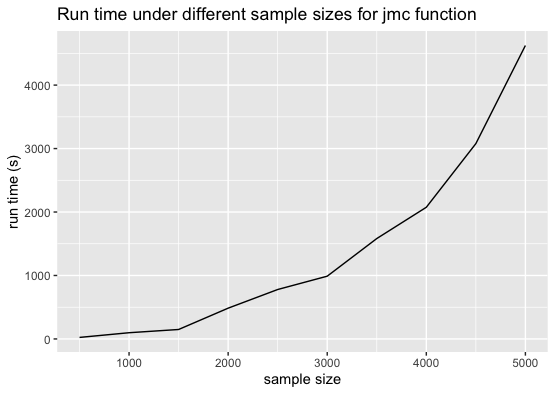
\includegraphics[width=8cm]{Fig1.png}
\centering
\caption{Run time comparison under different sample sizes for \texttt{jmc()} function (from 500 to 5000). Data setup: $p$ = 4, $n_q = 6$, 10.4\% censoring, 51.4\% risk 1, and 38.2\% risk 2. The run time under each sample size was based on one random sample.}
\label{fig:f1}
\end{figure}

\begin{figure}[!ht]
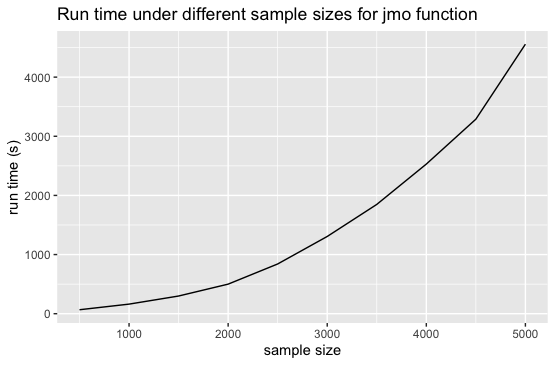
\includegraphics[width=8cm]{Fig2.png}
\centering
\caption{Run time comparison under different sample sizes for \texttt{jmo()} function (from 500 to 5000). Data setup: $p$ = 4, $n_q = 10$, 22.4\% censoring, 57.2\% risk 1, and 20.4\% risk 2. The run time under each sample size was based on one random sample.}
\label{fig:f2}
\end{figure}


\subsection{Data Simulation}
A simulation can generate datasets with exact ground truth for evaluation. Hence, the simulation of longitudinal and survival data with multiple failures associated with random effects is an important measure to assess the performance of joint modeling approaches dealing with competing risks. In  \textbf{JMcmprsk}, simulation tools are based on the data models proposed in \cite{elashoff2008joint} and \cite{li2010joint}, which can be used for testing joint models with continuous and ordinal longitudinal outcomes, respectively.

The main function for simulation data continuous longitudinal outcomes and survival data with multiple event outcomes is called \texttt{SimDataC()}, which has the following usage:
\begin{example}
SimDataC(k_val, p1_val, p1a_val, p2_val, g_val, truebeta, truegamma,
  randeffect, yfn, cfn, mfn)
\end{example}
We briefly explain some of the important options.\texttt{ k\_val} denotes the number of subjects in study;
\texttt{p1\_val} and \texttt{p1a\_val }denote the dimension of fixed effects and random effects in longitudinal measurements, respectively;  \texttt{p2\_val} and \texttt{g\_val} denotes the dimension of fixed effects and number to competing risks in survival data; \texttt{truebeta} and \texttt{truegamma} represent the true values of fixe effects in the longitudinal and  the survival submodels, respectively.  \texttt{randeffect} sets the true values for random effects in longitudinal and competing risks parts, namely in the order of $\sigma$,$\sigma_b$,$\nu_2$, and $\sigma_u$.

The following example generates the datasets used in simulation study in \cite{elashoff2008joint}:
\begin{example}
require(JMcmprsk)
set.seed(123)
yfn="jmcsimy1.txt";
cfn="jmcsimc1.txt";
mfn="jmcsimm1.txt";
k_val=200;p1_val=4;p1a_val=1; p2_val=2;g_val=2;
truebeta=c(10,-1,1.5,0.6);truegamma=c(0.8,-1,0.5,-1); randeffect=c(5,0.5,0.5,0.5);
#writing files
SimDataC(k_val, p1_val, p1a_val, p2_val, g_val,truebeta,
         truegamma, randeffect, yfn,  cfn,  mfn)
\end{example}
The output of function \texttt{SimDataC()} contains additional censoring rate information and newly generated files names for further usage.
\begin{example}
$`censoring_rate`
[1] 0.21
$rate1
[1] 0.45
$rate2
[1] 0.34
$yfn
[1] "jmcsimy1.txt"
$cfn
[1] "jmcsimc1.txt"
$mfn
[1] "jmcsimm1.txt"
\end{example}
The main function for data simulation with ordinal longitudinal outcomes and survival data with multiple event outcomes is called \texttt{SimDataO()}, the usage of which is very similar to \texttt{SimDataC()}:
\begin{example}
SimDataO(k_val, p1_val, p1a_val, p2_val, g_val, truebeta, truetheta,
  truegamma, randeffect, yfn, cfn, mfn)
\end{example}
All options have the same meanings as in \texttt{SimDataC()}, while \texttt{SimDataO()} has one more option \texttt{truetheta}, which sets the true values of the non-proportional odds longitudinal coefficients subset.

The following example generates the datasets used in simulation study in \cite{li2010joint}:
\begin{example}
require(JMcmprsk)
set.seed(123)
yfn="jmosimy1.txt";
cfn="jmosimc1.txt";
mfn="jmosimm1.txt";
 k_val=500;p1_val=3;p1a_val=1; p2_val=2;g_val=2;
truebeta=c(-1,1.5,0.8);truetheta=c(-0.5,1);truegamma=c(0.8,-1,0.5,-1); randeffect=c(1,0.5,0.5);
#writing files
SimDataO(k_val, p1_val, p1a_val, p2_val, g_val,
      truebeta, truetheta, truegamma, randeffect, yfn,  cfn,  mfn)
\end{example}
The output of the above function is
\begin{example}
$`censoring_rate`
[1] 0.218
$rate1
[1] 0.414
$rate2
[1] 0.368
$yfn
[1] "jmosimy1.txt"
$cfn
[1] "jmosimc1.txt"
$mfn
[1] "jmosimm1.txt"
\end{example}



\section{Conclusions and Future Work}
In this paper, we have illustrated the capabilities of package \textbf{JMcmprsk} for fitting joint models of time-to-event data with competing risks for two types of longitudinal data. We also present simulation tools to generate joint model datasets under different settings. Several extensions of \textbf{JMcmprsk}  package are planned to further expand on what is currently available. First, as the integral over the random effects becomes computationally burdensome in the case of high dimensionality, Laplace approximations or other Gauss-Hermite quadrature rules would be applied to the E-M step to speed up the computation procedure. Second, with the increasing need for predictive tools for personalized medicine, dynamic predictions for the aforementioned joint models will be added. Third, other new joint models such as joint analysis for bivariate longitudinal ordinal outcomes will be included.



\section{Acknowledgements}
We thank the reviewers for their insightful and constructive comments that led to significant improvements in our paper. The research of Hong Wang was partly supported by the National Social Science Foundation of China (17BTJ019). The research of Gang Li was partly supported by the National Institute of Health Grants P30 CA-16042, UL1TR000124-02, and P01AT003960.

\bibliography{wang-li-li-li}

\address{Hong Wang\\
  School of Mathematics \& Statistics,Central South University \\
  Changsha, Hunan Provinice,410075\\
  China\\
  \email{wh@csu.edu.cn}}

\address{Ning Li\\
  UCLA Biomathematics\\
  Los Angeles, CA 90095-1772\\
  USA\\
  \email{nli@biomath.ucla.edu}}

\address{Shanpeng Li\\
  Department of Biostatistics,UCLA School of Public Health\\
  Los Angeles, CA 90095-1772\\
  USA\\
  \email{lishanpeng0913@ucla.edu}}

\address{Gang Li*\\
  Department of Biostatistics,UCLA School of Public Health\\
  Los Angeles, CA 90095-1772\\
  USA\\
  (Corresponding Author)\\
  \email{vli@ucla.edu}}
